\documentclass{beamer}
%Information to be included in the title page:
\title{La felicità nel mondo}
\subtitle{Visualizzazione scientifica dei dati}
\author{Gabriele Bellini}
\institute{UNIMI}
%\date{}
\usetheme{Madrid}
\hypersetup{colorlinks=true,urlcolor=blue,linkcolor=white}


\usepackage{tikz}
\usetikzlibrary{calc}
\setbeamertemplate{background}{%
	\begin{tikzpicture}[remember picture,overlay]
	\node at (current page.center) [opacity=0.2, align=center] {\Huge\textbf{Copia non definitiva} \\ \textbf{Rilascio previsto per 07/07/23}};
	\end{tikzpicture}
}


\begin{document}
\frame{\titlepage}
\begin{frame}
	\frametitle{Il dataset}
	\begin{itemize}
		\item Raccoglie 10 anni di pubblicazioni
		\item La raccolta è stata assemblata da SimonaAsm
		\item I dati sono reperibili pubblicamente a \href{https://www.kaggle.com/datasets/simonaasm/world-happiness-index-by-reports-2013-2023}{Kaggle} 
		\item Licence: CDLA-Permissive-1.0
	\end{itemize}
	
\end{frame}

\begin{frame}
	\frametitle{Struttura del dataset}
	\begin{table}
		\centering
		\begin{tabular}{|l|l|l|l|}
			\hline
			PAESE & ANNO & FELICIT\'A & GRADUATORIA\\ \hline
			Afghanistan & 2013 & 4.04 & 143
\\
			Afghanistan & 2015 & 3.575 & 153
\\
			Afghanistan & 2016 & 3.36 & 154
\\
			Afghanistan & 2017 & 3.794 & 141
\\
			Afghanistan & 2018 & 3.632 & 145
\\
			Afghanistan & 2019 & 3.203 & 154
\\
			Afghanistan & 2020 & 2.567 & 153
\\
			Afghanistan & 2021 & 2.523 & 149
\\
			Afghanistan & 2022 & 2.404 & 146
\\
			Afghanistan & 2023 & 1.859 & 137
\\
			Albania & 2013 & 5.55 & 62
\\
			Albania & 2015 & 4.959 & 95 \\
			Albania & 2016 & 4.655 & 109 \\
			... & ... & ... & ... \\
			Zimbabwe & 2023 & 3.204 & 134\\
			\hline
		\end{tabular}
	\end{table}
\end{frame}

\begin{frame}{Le pubblicazioni contenute}
	\begin{itemize}
		\item Sono fatte dal \href{https://www.unsdsn.org/}{ Sustainable Development Solutions Network}\footnote{un'iniziativa globale delle Nazioni Unite (ONU)}
		\item Continene la media triennale dei dati sulla felicità
		\begin{itemize}
			\item es: il World Happiness Report del 2013 fornisce i coefficienti di 156 continenti calcolati sulla base del loro indice di felicità nel periodo 2010-2012
		\end{itemize}
	\item Il report usa dati del \href{https://www.gallup.com/topic/world-poll.aspx}{Gallup World Poll}\footnote{American Institute of Public Opinion, famoso per la raccolta di opinioni pubbliche in tutto il mondo}
	\end{itemize}
\end{frame}

\begin{frame}{Il calcolo dell'happiness index - La raccolta dati}
	I dati per il World Happiness Report vengono \textbf{raccolti tramite sondaggi} sulla felicità e benessere, nonché \textbf{attraverso fonti statistiche ufficiali} come dati economici, sanitari e sociali
\end{frame}

\begin{frame}{Il calcolo dell'happiness index - Le interviste}
	\begin{itemize}
		\item \textbf{[Il contenuto dei sondaggi]} Mettiamoci nei panni di un intervistato, la domanda che ci verrà chiesto di rispondere sarà: \\
		"Valuta la tua vita di oggi su una scala da 0 a 10, dove 10 rappresenta la miglior vita possibile e 0 la peggiore"
		\item \textbf{[Le metodologie di raccolta]} Se almeno l'80\% della popolazione è raggiungibile dalla linea telefonica le interviste si tengono tramite chiamate randomizzate altrimenti tramite visite porta a porta.
	\end{itemize}
\end{frame}

\begin{frame}{Aspetti statistici}
	\begin{itemize}
		\item Per ogni paese vengono effettuati 1000 \textbf{campionamenti} annui (3000 su 3 anni)
		\item l'index ha quindi un \textbf{intervallo di confidenza} del 95\%
	\end{itemize}
\end{frame}

\begin{frame}{Calcolo dell'happiness index - Le basi teoriche}
	L'indice è calcolato sulla base delle seguenti categorie
	\begin{itemize}
		\item PIL procapite (ricchezza)
		\item Supporto sociale (famiglia, amici, comunità)
		\item Aspettativa di vita in salute
		\item Libertà nelle scelte di vita
		\item Generosità
		\item Corruzione percepita
	\end{itemize}
	in comparazione con l'immaginaria Distopia
\end{frame}

\begin{frame}{Perché usare solo i 6 fattori per motivare}
	\begin{itemize}
		\item Hanno cercato di creare un indice che avesse un alto valore di \textbf{confrontabilità piuttosto che di causalità}
		\item Esisterebbero dati altrettanto importanti (es: disoccupazione, diseguaglianze) ma non sono reperibili per tutti i paesi
	\end{itemize}
\end{frame}

\begin{frame}{Cosa stiamo per osservare}
	Nei grafici che andremo a mostrare ci preoccuperemo di \textbf{come variano nel tempo} questi indici e \textbf{non sulle composizioni del singolo indice}
	\begin{itemize}
		\item Ad esempio non arriveremo a conclusioni come "happy people are overall healthier" (come si può leggere nel report del 2013)
	\end{itemize}
\end{frame}

\begin{frame}{Medie annue mondiali}
	\begin{figure}
		\centering
		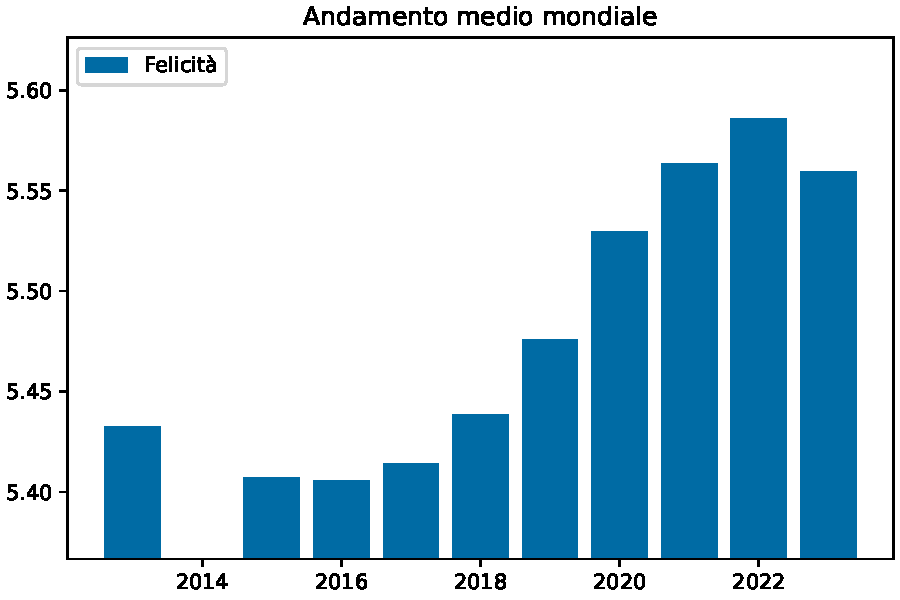
\includegraphics[width=0.75\textwidth]{"./img/1medieAnnue.pdf"}
		\caption{Immagine PDF con tutta la bellissima descrizione Immagine PDF con tutta la bellissima descrizione Immagine PDF con tutta la bellissima descrizione Immagine PDF con tutta la bellissima descrizione }
		\label{fig:pdf}
	\end{figure}
\end{frame}

\begin{frame}{Distribuzione di popolazione}
	\begin{figure}
		\centering
		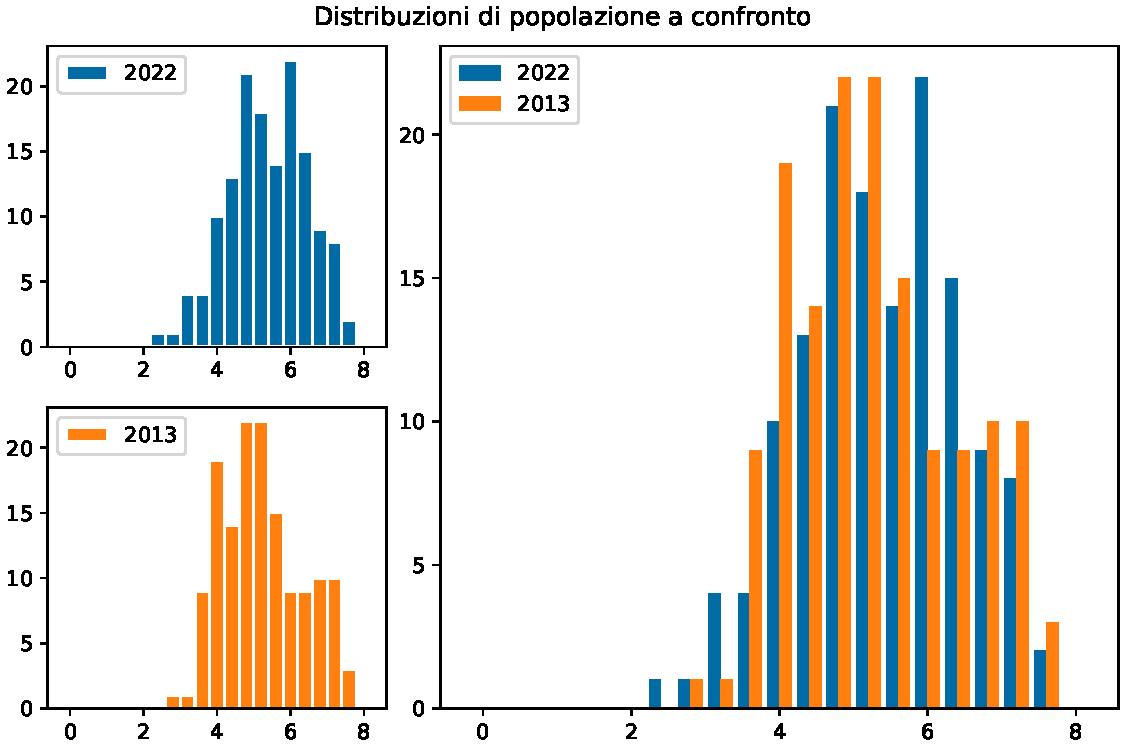
\includegraphics[width=0.75\textwidth]{"./img/2DistribuzioniPopolazioni.pdf"}
		\caption{Immagine PDF con tutta la bellissima descrizione Immagine PDF con tutta la bellissima descrizione Immagine PDF con tutta la bellissima descrizione Immagine PDF con tutta la bellissima descrizione }
		\label{fig:pdf}
	\end{figure}
\end{frame}

\begin{frame}{Comparazione 3 paesi IT FR GR}
	\begin{figure}
		\centering
		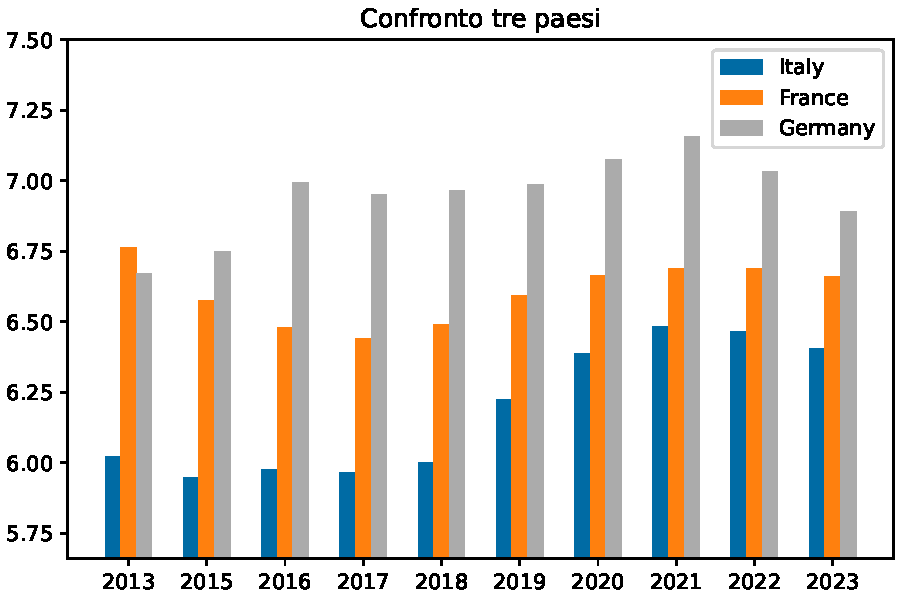
\includegraphics[width=0.75\textwidth]{"./img/3ComparoPaesi_Italy_France_Germany.pdf"}
		\caption{scasc}
	\end{figure}
\end{frame}

\begin{frame}{Comparazione 3 paesi TW HK CN}
	\begin{figure}
		\centering
		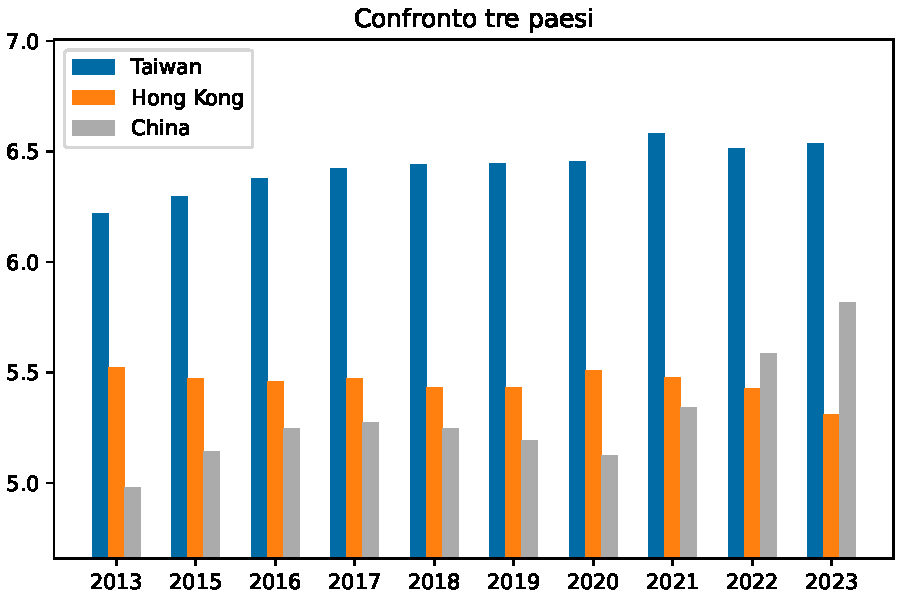
\includegraphics[width=0.75\textwidth]{"./img/3ComparoPaesi_Taiwan_HongKong_China.pdf"}
		\caption{scasc}
	\end{figure}
\end{frame}

\begin{frame}{Comparazione 3 paesi UA RU CN}
	\begin{figure}
		\centering
		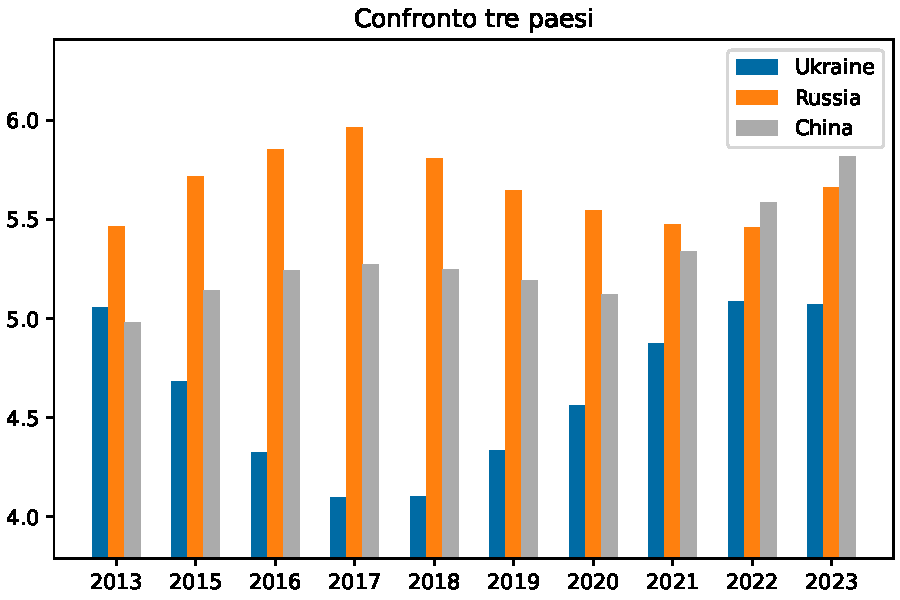
\includegraphics[width=0.75\textwidth]{"./img/3ComparoPaesi_Ukraine_Russia_China.pdf"}
		\caption{scasc}
	\end{figure}
\end{frame}

\begin{frame}{Continente Nord America 2022}
	\begin{figure}
		\centering
		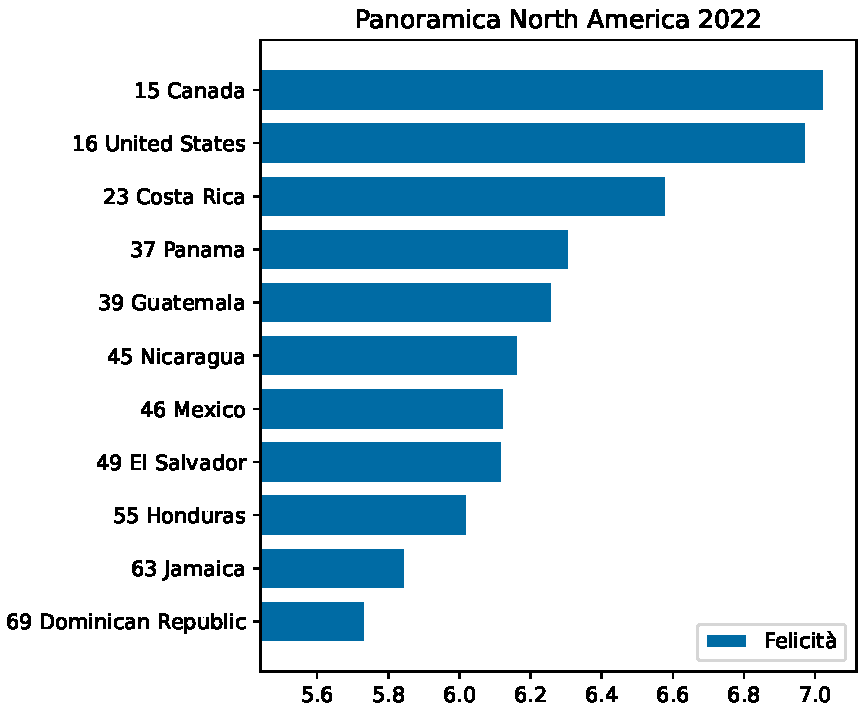
\includegraphics[width=0.75\textwidth]{"./img/4Classifica_North America_2022.pdf"}
		\caption{scasc}
	\end{figure}
\end{frame}

\begin{frame}{Continente Sud America 2022}
	\begin{figure}
		\centering
		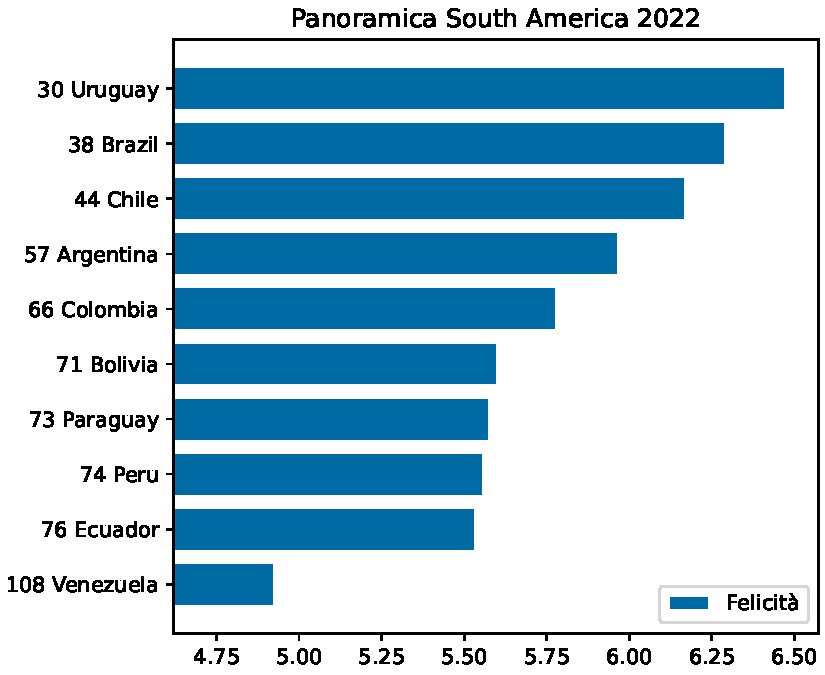
\includegraphics[width=0.75\textwidth]{"./img/4Classifica_South America_2022.pdf"}
		\caption{scasc}
	\end{figure}
\end{frame}

\begin{frame}{Andamenti nel tempo per continente}
	\begin{figure}
		\centering
		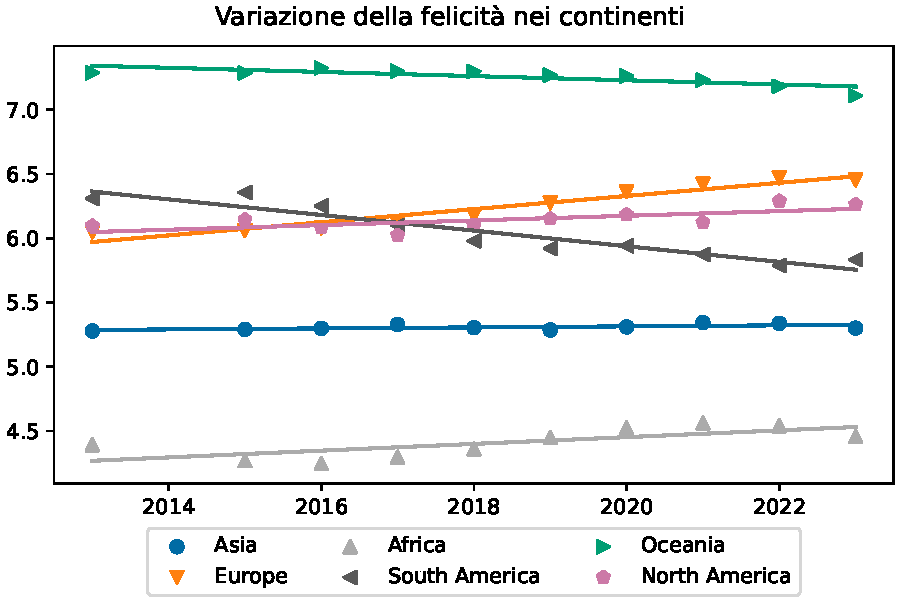
\includegraphics[width=0.75\textwidth]{"./img/5AndamentiContinentali.pdf"}
		\caption{scasc}
	\end{figure}
\end{frame}
%------------------------
\begin{frame}{Paesi con maggiori variazioni dal 2011}
	\begin{figure}
		\centering
		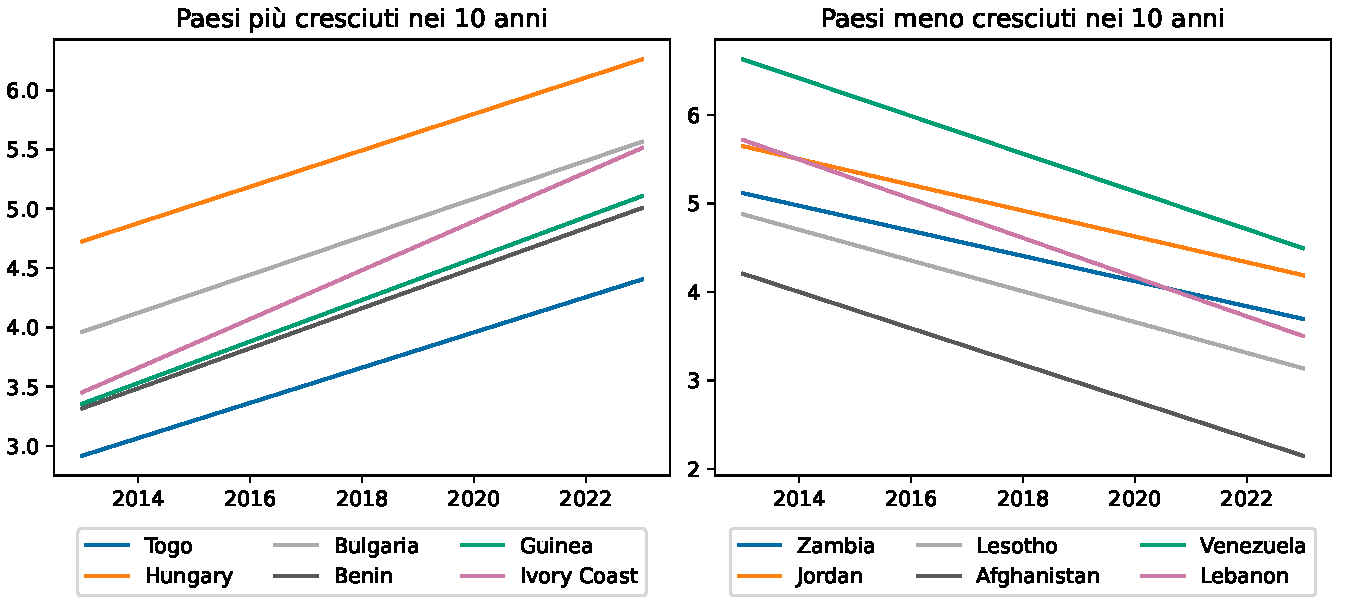
\includegraphics[width=1\textwidth]{"./img/6MaggioreVariazione.pdf"}
		\caption{scasc}
	\end{figure}
\end{frame}

\begin{frame}{Chi è più portato alla crescita, chi stava meglio o peggio?}
	\begin{figure}
		\centering
		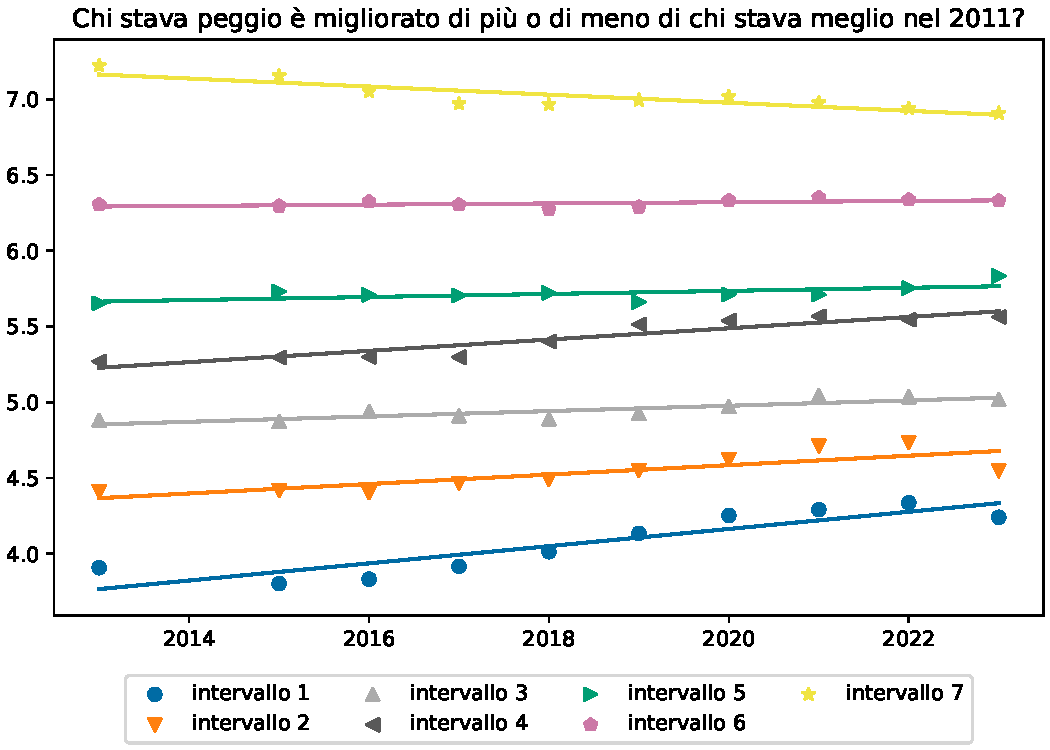
\includegraphics[width=0.75\textwidth]{"./img/7ImmobilismoOVariazioneBenessere.pdf"}
		\caption{scasc}
	\end{figure}
\end{frame}
% distribuzioni di popolazioni a confronto
% confronto a 3 paesi
% Continente NOME ANNO
% ultimo e penultimo triooi ouccolo

\end{document}